\chapter{Exploring $N = 3$ with a Leapfrog Algorithm}

With a better algorithm in hand, our friends decided to work their way
up from the two-body problem to the three-body problem.  And rather
than hard coding the value of $N$ in their algorithm, they wrote a
leapfrog code for the general $N$-body problem.  The expression for
the acceleration felt by particle $i$ is given by summing together the
Newtonian gravitational attraction of all other particles $j$, where
both $i$ and $j$ take on values from 1 up to and including $N$:

\begin{equation}
\frac{d^2}{dt^2}\br_i =  G \sum_{j=1 \atop j \neq i}^N M_j
\frac{\br_j - \br_i}{\,|\br_j - \br_i|^3}
\end{equation}

\noindent
Here $M_j$  and $\br_j$ are the mass and position vector of particle $j$,
and $G$ is the gravitational constant.  To bring out the inverse square
nature of gravity, we can define $\br_{ji} = \br_j - \br_i$, with
$r_{ji} = |\br_{ji}|$, and unit vector $\hat \br_{ji} = \br_{ji} / r_{ji}$:

\begin{equation}
\ba_i = G \sum_{j=1 \atop j \neq i}^N
\frac{M_j}{r_{ji}^2} \,\hat\br_{ji}\label{newton}
\end{equation}

\noindent
Note that the summation excludes self-interactions: every particle
feels the forces of the other $N-1$ particles, but not its own force
(which would be infinitely large in case of a point mass).

\section{A More General Leapfrog}

For simplicity, Alice {\it et al.} decided to continue to embed the
initial conditions at the beginning of their code, leaving until later
the task of writing a more general input routine.  It contains initial
conditions corresponding to three particles moving equidistantly on a
circle.  Here is the code they produced.  We will look at the
different parts in turn in the following sections.

\code{leapfrog2.C}{chap5/leapfrog2.C}

Not surprisingly, the $N$-body code {\st leapfrog2.C} is more than
twice as long as the code {\st leapfrog1.C} which was hardwired for
$N=2$.  The general lay-out is similar, so we will quickly walk
through it, pointing out the salient differences.

One new feature is the expression {\st const} in front of the
declaration of the two variables {\st m} and {\st pi}.  In C++ this
means that you cannot change the value, once you have assigned it.  If
you would try to change the value of a {\st const} variable, the
compiler would issue an error message.  But apart from making code
maintenance safer by preventing someone from changing a value that
should not be changed by mistake, it also makes the code more easy to
read, since it tells the human reader that there is a reason to keep a
particular value constant.

In our case, we have chosen to give all particles the same mass, and
we do not want particles to lose or gain mass, and therefore we
declare and initialize the variable storing the shared mass value as
{\st const double m = 1}.  The variable {\st pi} stands for the
mathematical constant $\pi = 3.14159\dots$, and is therefore declared
as {\st const double pi = 2 * asin(1)}.  The actual value is obtained
from the arc sine function {\st asin()}, which is defined as the
inverse of the sine function: when $y = \sin(x)$, then $x=\arcsin(y)$.
Since $\sin(\pi/2)=1$, we have $pi = 2 \arcsin(1)$.

\section{Coordinates in the Center of Mass System}

Unlike the two-body case, there is no gain in simplicity if we would
use relative coordinates for the $N$-body system in general.  For two
bodies, there is only one set of relative coordinates, while there
are two sets of particle coordinates, one for each particle.  For
three bodies, there are three combinations of separations between
individual particles, just as there are three sets of particle
coordinates.  In that case, it is a matter of taste which one one
prefers to use.  For all higher values of $N$, the number of relative
separations is always larger than the number of particles (six versus
four for $N=4$, for example).  In conclusion, from $N=3$ onward,
it makes more sense to define the positions and velocities with
respect to a given coordinate system.

Although not necessary, it is often convenient to use the center of
mass system for our orbit calculations.  The center of mass is defined
in any coordinate system as

\begin{equation}
\bR = \frac{1}{M} \sum_{i=1}^N m_i\br_i \label{com-pos}
\end{equation}

\noindent
where $N$ is the total number of particles, $m_i$ and $\br_i$ are the
mass and the position of particle $i$, and $M=\sum_{i=1}^N m_i$ is the
total mass of the system.  We can interpret the right hand side as a
type of lever arm equation.  In a one-dimensional system of weights
hanging from a beam in the Earth's gravitational field, the left and
right parts of the beam will be in equilibrium if we support the beam
exactly at the center of mass.  The same is true for a two-dimensional
plank with masses.

With three dimensions, we have no room left in an extra dimension for
external support, but an analogous result still holds: the motion of
the center of mass is the same as if the entire mass of the system was
concentrated there and acted upon by the resultant of all external
forces.  See any textbook on classical dynamics for a derivation of
this property.  In the case of an isolated $N$-body system, there are
no external forces, and therefore the center of mass will move in a
straight line.

Starting with a given coordinate system, and subtracting the center of
mass position vector $\bR$ from all particle positions allows us to
construct a representation of the $N$-body system in its c.o.m. system
(a short hand for `center of mass').  Subtracting the c.o.m. position
is not enough, however.  While this causes a momentary centering, it
is still quite possible that the $N$-body will start drifting off soon
thereafter.  To keep the system in place, at least on average, we also
have to subtract the velocity of the c.o.m. $\bV$ from all particle
velocities.  Differentiation of Eq. \ref{com-pos} gives:

\begin{equation}
\bV = \frac{1}{M} \sum_{i=1}^N m_i\bv_i \label{com-vel}
\end{equation}

\noindent
This shows, incidentally, that the total momentum of all particles is
zero in the c.o.m. coordinate system.  Since the c.o.m. moves in a
straight line, no further corrections are necessary.  Throughout this
book, when we set up initial conditions for an $N$-body system, we
will do so in the c.o.m. of that system.

At the beginning of our code, we see how positions, velocities, and
accelerations are now represented by two-dimensional arrays, where the
first counter indicates the number of the particle in an $N$-body
system, and the second counter the Cartesian coordinate.  Note that in
C++ array counters start at zero.  Therefore, the $y$ component of the
position of the 3rd particle is not stored in {\st a[3][2]} as one might
naively think, but rather in {\st a[2][1]}.  In a 3-body system such as
the one coded here, the value {\st a[3][2]} is in fact undefined, since it
lies outside the memory area assigned to the area; using that value
would present a serious bug.

\section{Setting up Three Stars on a Circle}

Although our code is written so as to function for an arbitrary number
of particles, we initialize only three particles at the beginning of
{\st leapfrog2.C}.  This can be easily changed to a larger number of
particles in different configurations.  A few chapters later we will
see how to read in an arbitrary $N$-body configuration.

It was Bob who was curious to see what happened when we place three
stars equally spaced along a circle.  After he had coded up the
two-body leapfrog, which showed him how stable a two-body orbit of two
particles was, he asked Alice whether a three body configuration would
be equally stable.  She said it wouldn't, and they all agreed that it
would be fun to see for themselves.  For simplicity, they gave all
particles the same mass {\st m = 1}.

Anticipating that the instability might take some time to develop,
they decided to add one other input option, besides the time step {\st
dt}, namely the total duration of the run {\st t\_end}, as we can see
in the code.  Directly below that request, we see how they spaced the
three stars around the unit circle.  The first star was chosen to
reside at distance unity along the positive $x$ axis, implying a
position vector $\br = \{1,0,0\}$.  With the condition that the motion
takes place in the $\{x,y\}$ plane, the position of the other two
stars is then fixed, as shown.

Following the position assignments, the accelerations are calculated.
As we saw before, we have to spin the wheels of the gravitational
acceleration module once, before we can safely enter the main
integration loop.  As far as the code is concerned, there is no
surprise here, given that we already figured out the overall structure
in the two-body case.  The only thing new, apart from the use of
two-dimensional arrays, is the double loop over all particles in the
system.  The outer loop once visits each particle $i$, while the inner
loop visits only those particles $j$ for which $j>i$.  At the end of
the loop the accelerations of particles $i$ and $j$ on each other are
calculated.  The reason to avoid $j=i$ is that the particles show no
self-attraction.  The reason to skip $j<i$ is a matter of efficiency:
once we have calculated the intermediate quantities needed to
calculate {\st a[j][k]}, the acceleration of particle $j$ caused by
the gravitational attraction of particle $i$, we may as well calculate
{\st a[j][k]} on the spot, which is the acceleration of particle $i$
caused by the gravitational attraction of particle $j$.  In our
equal-mass case the two are in fact equal in magnitude and opposite in
sign, but in the more general case where the two masses are unequal,
we would introduce a mass array, and write:

\begin{small}
\begin{verbatim}
                a[i][k] += m[j] * rji[k] / r3;
                a[j][k] -= m[i] * rji[k] / r3;
\end{verbatim}
\end{small}

The next group of lines employs a shortcut in order to determine the
initial velocities of the three particles.  Since an $N$-body system
is governed by second order differential equations, we have to supply
positions and velocities for all particles as initial conditions
before we can start to solve the equations of motion, which give us
the accelerations.  In order to guarantee that our three stars start
off on a circular motion, we use the fact that the centrifugal
acceleration in a uniform circular orbit is given by $v^2/r$.  Since
the gravitational centripetal acceleration has to balance the
centrifugal acceleration, we can solve for $v$, the magnitude of the
velocity, once we know $a$, the magnitude of the gravitational
acceleration, a quantity that is equal by symmetry for all three
particles, as is $v$ and $r$.  We find $v = \sqrt{ar}$.

In our case, the magnitude of the position of each star was chosen to
be unity.  Therefore, the magnitude of the velocities are $v = \sqrt{a}$.
The direction of the velocity of the first particle is chosen to lie
along the positive $y$ axis.  This choice determines the other two
velocities {\st v[1][]} and {\st v[2][]} by successive rotations over
120 degrees, or $2 \pi / 3$ (by the way, while it is nice to let the
computer do all the calculating, it is not difficult to derive with
pen and paper that in our case $a = 1\sqrt{3}$ and thus $v = 3^{-1/4}$).

The rest of the code is again a straightforward generalization of the
two-body case.  Like we did before, we compute the total energy before
and after the full orbit integration.  Note that we could have folded
the calculation of the potential energy in with the calculation of the
initial accelerations.  Doing so would make the program somewhat
shorter, but it would make the logical structure less easy to
understand.  There would be no gain in overall efficiency either,
since almost all the compute happens in the {\st for} loop which gets
traversed thousands or more times.  In comparison, what happens only
once before and after the orbit integration can be as inefficient as
we want and still not affect the total running time significantly.

\section{Looking for Instabilities}

Let us follow the conversation of Alice, Bob, and Carol, while they
are using {\st leapfrog2.C} as a laboratory tool to investigate the
stability of the behavior of three bodies initially moving uniformly
and equally space along a circle.  This time, Alice is behind the key
board.

\abc

\alice
Having finally debugged our new 3-body leapfrog code enough to keep
the compiler happy, let us now see how the three stars behave when we
launch them on a circle.  Here goes.

\cba

\begin{small}
\begin{verbatim}
|gravity> g++ -o leapfrog2 leapfrog2.C
|gravity> leapfrog2 > leapfrog2_0.01_10.out
Please provide a value for the time step
0.01
and for the duration of the run
10
Initial total energy E_in = -0.866025
Final total energy E_out = -0.866025
absolute energy error: E_out - E_in = 2.72254e-10
relative energy error: (E_out - E_in) / E_in = -3.14372e-10
|gravity>
\end{verbatim}
\end{small}

\abc

\bob
Wow, what a small energy error!  Clearly, our leapfrog code can run
circles around the forward Euler code.

\alice
What you see here is partly an artifact of going around a perfect
circle.  The leapfrog will do less well on an ellipse or on an
arbitrary orbit.  The symmetry of the circle together with the time
symmetry of the leapfrog helps to cancels errors.  So from the fact
that the energy errors are so small, I bet that we are still moving
happily around the initial circle.

\carol
I don't want to bet yet, but let us inspect.  Can you show us a
picture?

\cba

\begin{figure}[htb]
\centering
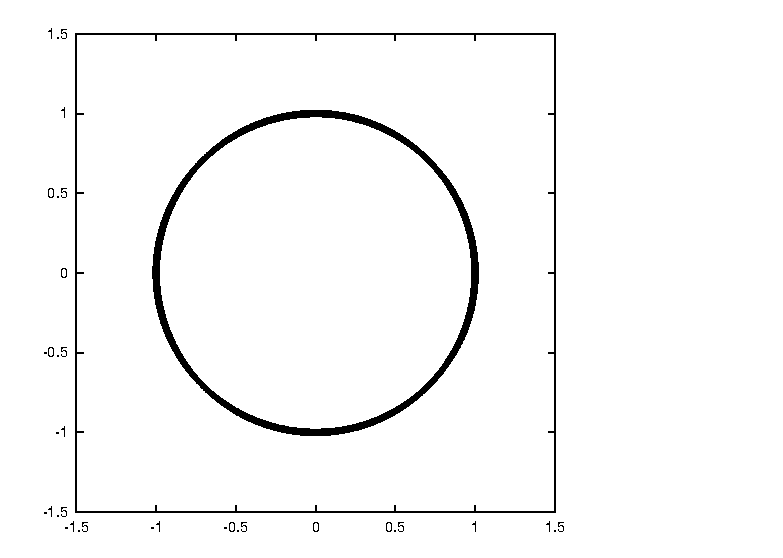
\includegraphics[width=2.5in]{chap5/leapfrog2_0.01_10.ps}
\caption[Three stars on a circle, leapfrog, $dt = 0.01$, $t_{end} = 10$]
{The first attempt to integrate the orbits of three stars
starting off on a circle, with time step $dt = 0.01$ and a total
duration of $t_{end} = 10$}
\label{fig:leap2-0.01-10}
\end{figure}

\abc

\bob
You are right, Alice, as far as moving on a circle goes.  Now I wonder
whether you were right about the stars developing an instability.  It
doesn't look like it --- so far!

\alice
Only one way to find out:

\cba

\begin{small}
\begin{verbatim}
|gravity> leapfrog2 > leapfrog2_0.01_100.out
Please provide a value for the time step
0.01
and for the duration of the run
100
Initial total energy E_in = -0.866025
Final total energy E_out = -0.86602
absolute energy error: E_out - E_in = 5.63203e-06
relative energy error: (E_out - E_in) / E_in = -6.5033e-06
|gravity>
\end{verbatim}
\end{small}

\begin{figure}[htb]
\centering
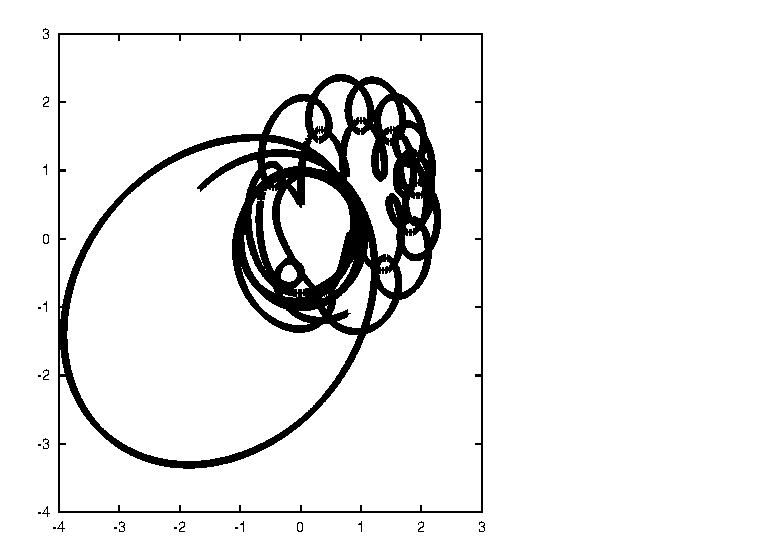
\includegraphics[width=2.5in]{chap5/leapfrog2_0.01_100.ps}
\caption[Three stars on a circle, leapfrog, $dt = 0.01$, $t_{end} = 100$]
{The second attempt to integrate the orbits of three stars
starting off on a circle, with time step $dt = 0.01$ and a total
duration of $t_{end} = 100$}
\label{fig:leap2-0.01-100}
\end{figure}

\abc

\bob
Okay, Alice seems to be right on both counts!  First of all, the
energy error is now ten thousand times larger, even though we ran only
ten times longer, so that confirms her circle argument.  But before I
congratulate her on the instability, I have one nagging question.
I wonder whether this fancy three-body dance is caused by numerical
instabilities caused by finite accuracy of the leapfrog, or whether it
is a physical instability which real stars would undergo?

\alice
I bet the latter, since we have not yet discovered even one such
system in the sky, even though we have found countless multiple stars,
from triples to quadruples and quintuples and up.  But why don't we
check?  Let's refine the time step a few times by an order of magnitude.

\cba

\begin{small}
\begin{verbatim}
|gravity> leapfrog2 > leapfrog2_0.001_100.out
Please provide a value for the time step
0.001
and for the duration of the run
100
Initial total energy E_in = -0.866025
Final total energy E_out = -0.866025
absolute energy error: E_out - E_in = 1.58819e-07
relative energy error: (E_out - E_in) / E_in = -1.83388e-07
|gravity>
\end{verbatim}
\end{small}

\begin{figure}[htb]
\centering
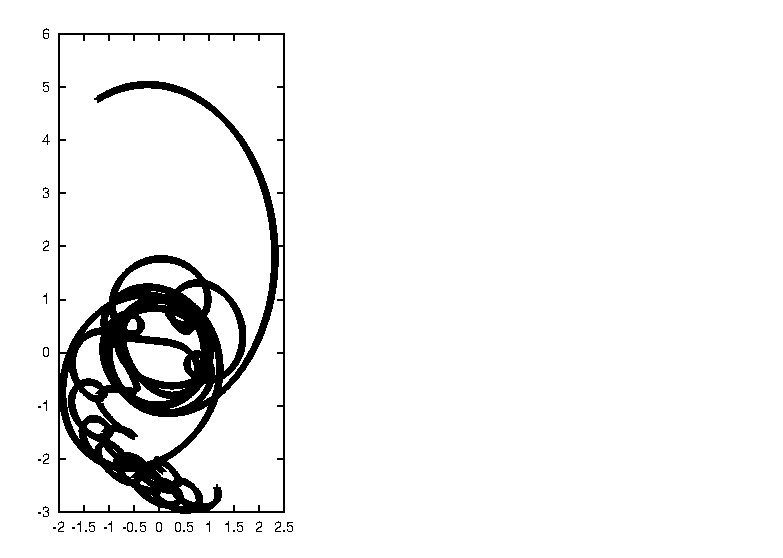
\includegraphics[width=2.5in]{chap5/leapfrog2_0.001_100.ps}
\caption[Three stars on a circle, leapfrog, $dt = 0.001$, $t_{end} = 100$]
{The third attempt to integrate the orbits of three stars
starting off on a circle, with time step $dt = 0.001$ and a total
duration of $t_{end} = 100$}
\label{fig:leap2-0.001-100}
\end{figure}

\begin{small}
\begin{verbatim}
|gravity> leapfrog2 > leapfrog2_0.0001_100.out
Please provide a value for the time step
0.0001
and for the duration of the run
100
Initial total energy E_in = -0.866025
Final total energy E_out = -0.866025
absolute energy error: E_out - E_in = 1.1609e-09
relative energy error: (E_out - E_in) / E_in = -1.3405e-09
|gravity>
\end{verbatim}
\end{small}

\begin{figure}[htb]
\centering
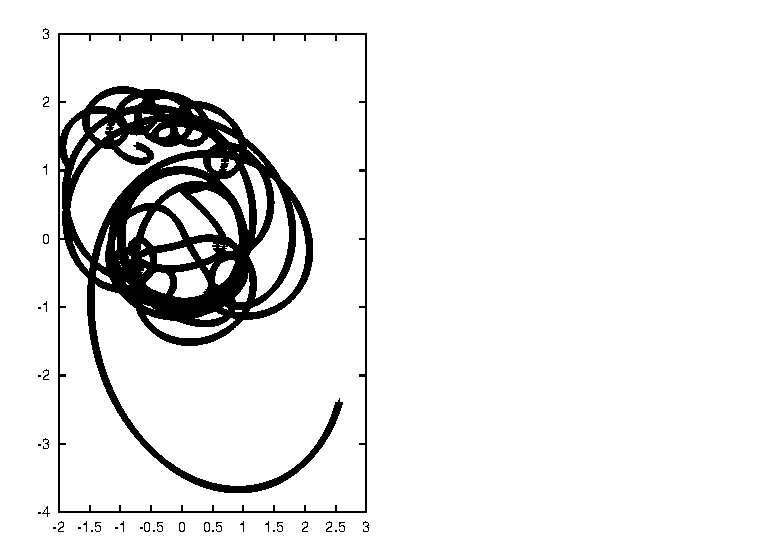
\includegraphics[width=2.5in]{chap5/leapfrog2_0.0001_100.ps}
\caption[Three stars on a circle, leapfrog, $dt = 0.0001$, $t_{end} = 100$]
{The fourth attempt to integrate the orbits of three stars
starting off on a circle, with time step $dt = 0.0001$ and a total
duration of $t_{end} = 100$}
\label{fig:leap2-0.0001-100}
\end{figure}

\abc

\bob
Well, Alice, what did I tell you?  Each picture is wildly different,
so I don't think that we are converging onto an actually existing
unstable orbit.

\alice
Well, let's try one more refinement.

\cba

\begin{small}
\begin{verbatim}
|gravity> leapfrog2 > leapfrog2_0.00001_100.out
Please provide a value for the time step
0.00001
and for the duration of the run
100
Initial total energy E_in = -0.866025
Final total energy E_out = -0.866025
absolute energy error: E_out - E_in = 1.17143e-10
relative energy error: (E_out - E_in) / E_in = -1.35265e-10
|gravity>
\end{verbatim}
\end{small}

\begin{figure}[htb]
\centering
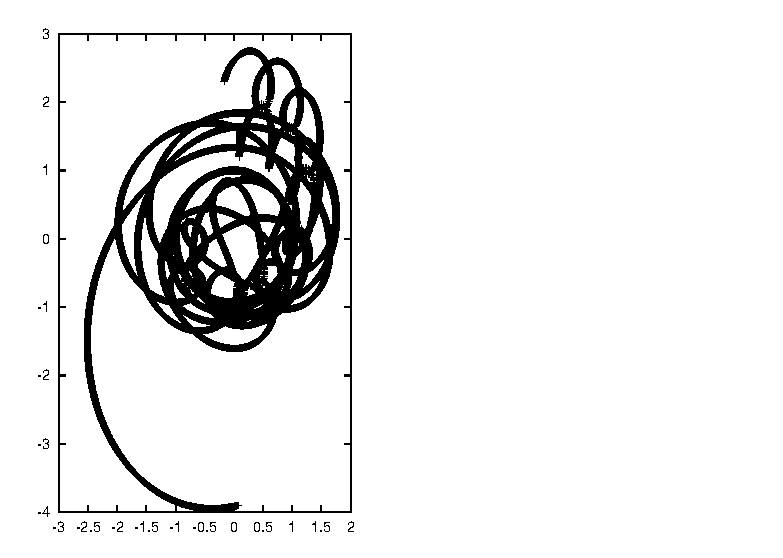
\includegraphics[width=2.5in]{chap5/leapfrog2_0.00001_100.ps}
\caption[Three stars on a circle, leapfrog, $dt = 0.00001$, $t_{end} = 100$]
{The fifth attempt to integrate the orbits of three stars
starting off on a circle, with time step $dt = 0.00001$ and a total
duration of $t_{end} = 100$}
\label{fig:leap2-0.00001-100}
\end{figure}

\abc

\alice
Well, at least the last two are somewhat similar, unlike all previous
pictures.  But alike they are certainly not.

\bob
Okay, one more refinement, and perhaps the whole thing will finally
converge!  With {\st dt = 0.000001}, this means a hundred million steps,
but why not, computers are fast enough these days.

\cba

\begin{small}
\begin{verbatim}
|gravity> leapfrog2 > leapfrog2_0.000001_100.out
Please provide a value for the time step
0.000001
and for the duration of the run
100
Initial total energy E_in = -0.866025
Final total energy E_out = -0.866025
absolute energy error: E_out - E_in = 8.68972e-13
relative energy error: (E_out - E_in) / E_in = -1.0034e-12
|gravity>
\end{verbatim}
\end{small}

\begin{figure}[htb]
\centering
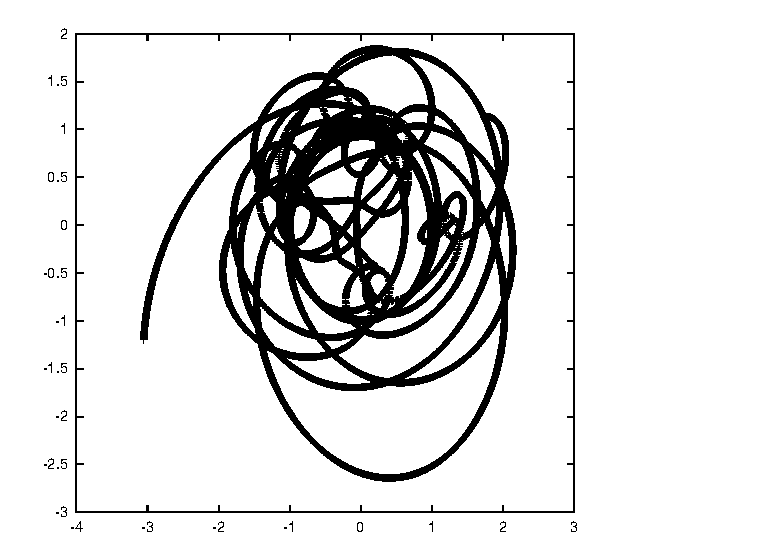
\includegraphics[width=2.5in]{chap5/leapfrog2_0.000001_100.ps}
\caption[Three stars on a circle, leapfrog, $dt = 0.000001$, $t_{end} = 100$]
{The sixth attempt to integrate the orbits of three stars
starting off on a circle, with time step $dt = 0.000001$ and a total
duration of $t_{end} = 100$}
\label{fig:leap2-0.000001-100}
\end{figure}

\abc

\bob
So much for similar but not alike.  This one doesn't look anything
like the previous one.  And we are rapidly approaching machine accuracy.

\alice
Hmmmm.

\cba

\section{Priming the Pump}

\abc

\carol
Hmmmm indeed.  Aha!  I have an idea.  Even if the instability exists
in the real world, it still has to be triggered in some way.  In our
computer it is triggered by round-off errors.  In the real world, if
we put a pencil on its tip straight up and let go, the pencil will
fall in a random direction, triggered by the Brownian motion of the
air molecules, even if we would have aligned it perfectly vertically.
Brownian motion is not reproducible, but neither can you expect
round-off errors to be reproducible when you change time steps.

\alice
Interesting point!  Let us try.  Let us give one of the stars a little
perturbation in its velocity, on the order of $10^{-4}$, huge compared
to the round-off noise around $10^{-15}$, but still larger than typical
numerical errors of the leapfrog, certainly for small enough step size.
Okay, here is a version, {\st leapfrog2a.C}.  The only change I have
made with respect to {\st leapfrog2a.C} is the addition of one line,
immediately following the assignment of the velocities:

\cba

\begin{small}
\begin{verbatim}
    v[0][0] += 0.0001;
\end{verbatim}
\end{small}

\abc

\bob
I see.  You are priming the pump, to guide the instability.  And
you have put this line just after the velocity initialization,
so that it appears conveniently just before the first calculation of
the kinetic energy.  That way, the first total energy calculation
takes this displacement in the value of this one velocity component
into account.  By now, I do expect the system to fall apart again, and
I'm really curious.  If the resulting dance pattern jumps all over the
place again, we definitely are dealing with errors introduced by the
leapfrog.  But if we converge to one particular orbit, then I concede
that we have uncovered a physical instability, where a given
well-defined tiny displacement leads to a well-defined resulting way
in which the system falls apart.  Let's have a look, Alice!

\alice
I'll start again with only ten time units, to check that our
three stars complete at least a few orbits on their original circle,
before going their own way.

\cba

\begin{small}
\begin{verbatim}
|gravity> g++ -o leapfrog2a leapfrog2a.C
|gravity> leapfrog2a > leapfrog2a_0.01_10.out
Please provide a value for the time step
0.01
and for the duration of the run
10
Initial total energy E_in = -0.866025
Final total energy E_out = -0.866025
absolute energy error: E_out - E_in = 1.21321e-09
relative energy error: (E_out - E_in) / E_in = -1.40089e-09
|gravity>
\end{verbatim}
\end{small}

\abc

\bob
Applying Alice's detective strategy, I would say that the energy error
is still too small to show detectable deviations from a circle.
Notice that the error is clearly larger than before, as we would
expect, since we have given the instability a hand by starting
with a gentle push.

\alice
Elementary, my dear Bob.  But let us see whether you are right.

\cba

\begin{figure}[htb]
\centering
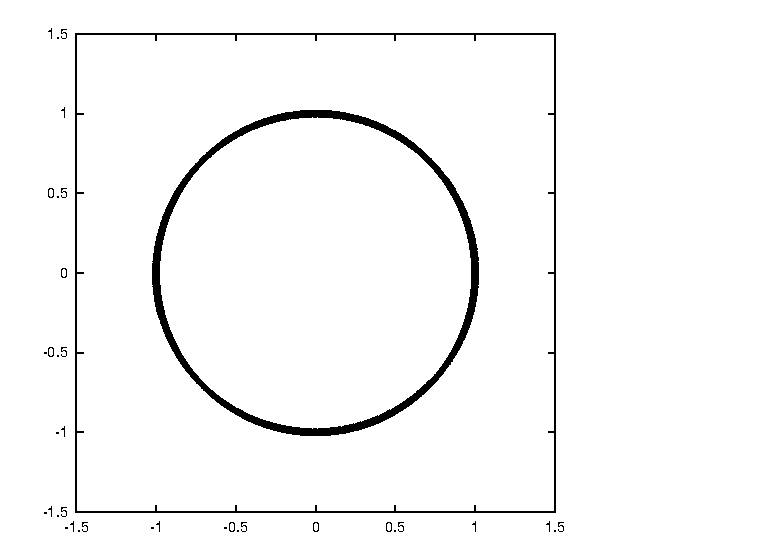
\includegraphics[width=2.5in]{chap5/leapfrog2a_0.01_10.ps}
\caption[Three stars on a circle, leapfrog, $dv_{init}=0.0001$, $dt = 0.01$,
$t_{end} = 10$]
{The first attempt to integrate the orbits of three stars
starting off on a circle with an initial velocity perturbation of 
$dv_{init}=0.0001$, time step $dt = 0.01$ and a total duration of
$t_{end} = 10$}
\label{fig:leap2a-0.01-10}
\end{figure}

\abc

\bob
Encouraged by my success in following Alice's footsteps,, I will now
predict a significant degradation in the energy conservation, together
with the appearance of a wild three-body dance, when we go to 100 time
units.

\alice
You should become my agent --- here are the run and the plot:

\cba

\begin{small}
\begin{verbatim}
|gravity> leapfrog2a > leapfrog2a_0.01_100.out
Please provide a value for the time step
0.01
and for the duration of the run
100
Initial total energy E_in = -0.866025
Final total energy E_out = -0.865241
absolute energy error: E_out - E_in = 0.000784568
relative energy error: (E_out - E_in) / E_in = -0.000905941
|gravity>
\end{verbatim}
\end{small}

\begin{figure}[htb]
\centering
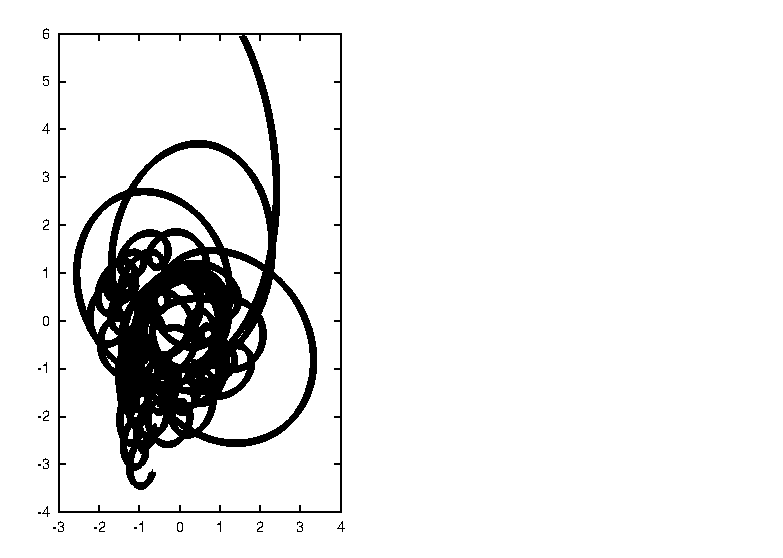
\includegraphics[width=2.5in]{chap5/leapfrog2a_0.01_100.ps}
\caption[Three stars on a circle, leapfrog, $dv_{init}=0.0001$, $dt = 0.01$,
$t_{end} = 100$]
{The second attempt to integrate the orbits of three stars
starting off on a circle with an initial velocity perturbation of 
$dv_{init}=0.0001$, time step $dt = 0.01$ and a total duration of
$t_{end} = 100$}
\label{fig:leap2a-0.01-100}
\end{figure}

\abc

\carol
I bet Bob didn't envision {\it such} a big degradation in energy
conservation!  Let's make the time steps a factor ten smaller.

\cba

\begin{small}
\begin{verbatim}
|gravity> leapfrog2a > leapfrog2a_0.001_100.out
Please provide a value for the time step
0.001
and for the duration of the run
100
Initial total energy E_in = -0.866025
Final total energy E_out = -0.866033
absolute energy error: E_out - E_in = -7.29447e-06
relative energy error: (E_out - E_in) / E_in = 8.42293e-06
|gravity>
\end{verbatim}
\end{small}

\begin{figure}[htb]
\centering
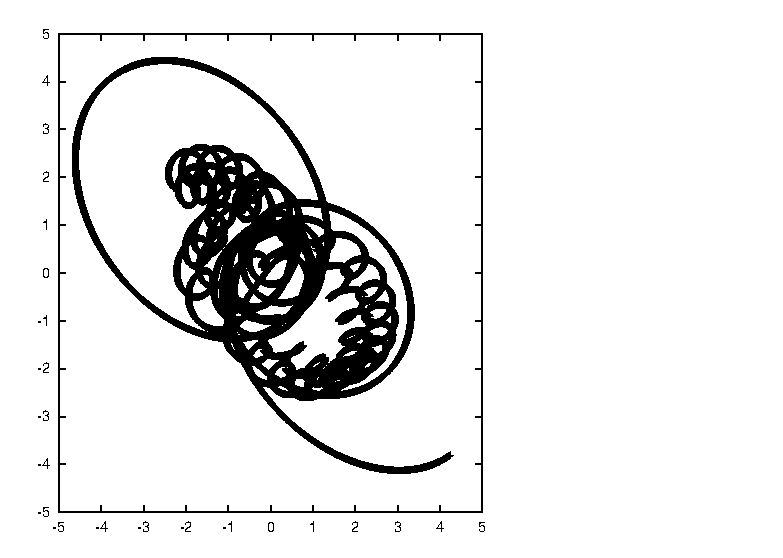
\includegraphics[width=2.5in]{chap5/leapfrog2a_0.001_100.ps}
\caption[Three stars on a circle, leapfrog, $dv_{init}=0.0001$, $dt = 0.001$,
$t_{end} = 100$]
{The third attempt to integrate the orbits of three stars
starting off on a circle with an initial velocity perturbation of 
$dv_{init}=0.0001$, time step $dt = 0.001$ and a total duration of
$t_{end} = 100$}
\label{fig:leap2a-0.001-100}
\end{figure}

\abc

\bob
You are right, I had expected an energy error more like the present
one, already in the previous round.

\alice
My hunch is that the previous round may have featured a particularly
close encounter.  Since our code does not know how to decrease the
time step during close encounters, even one such encounter can spoil
the energy conservation of a whole run.  At some point we'll have to
make our integrator smarter and more autonomous in the eye of danger.

\carol
But not now.  I want to see whether we will reach convergence.  So far
the last two pictures don't look any more like each other than in the
case before we primed the pump.  Can we refine the time step by
another order of magnitude?

\alice
Sure, my pleasure.

\cba

\section{Reaching Convergence}

\begin{small}
\begin{verbatim}
|gravity> leapfrog2a > leapfrog2a_0.0001_100.out
Please provide a value for the time step
0.0001
and for the duration of the run
100
Initial total energy E_in = -0.866025
Final total energy E_out = -0.866025
absolute energy error: E_out - E_in = 2.55083e-08
relative energy error: (E_out - E_in) / E_in = -4.10015e-08
|gravity>
\end{verbatim}
\end{small}

\begin{figure}[htb]
\centering
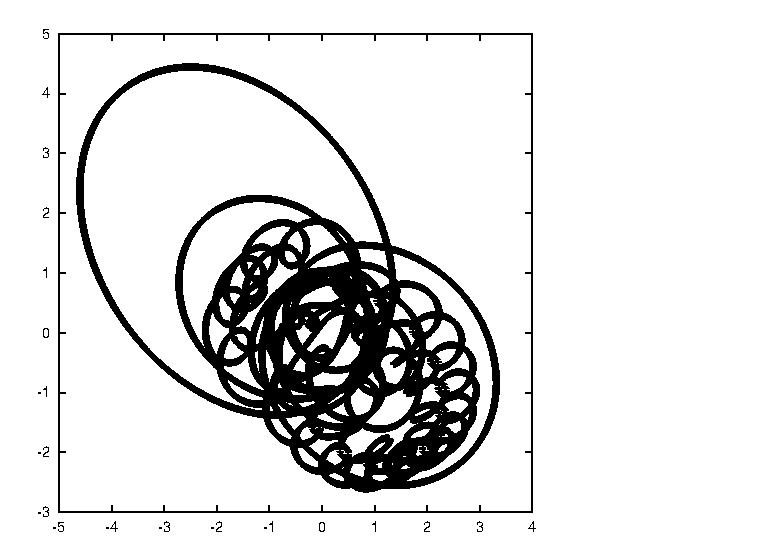
\includegraphics[width=2.5in]{chap5/leapfrog2a_0.0001_100.ps}
\caption[Three stars on a circle, leapfrog, $dv_{init}=0.0001$, $dt = 0.0001$,
$t_{end} = 100$]
{The fourth attempt to integrate the orbits of three stars
starting off on a circle with an initial velocity perturbation of 
$dv_{init}=0.0001$, time step $dt = 0.0001$ and a total duration of
$t_{end} = 100$}
\label{fig:leap2a-0.0001-100}
\end{figure}

\abc

\bob
Still quite different pictures.  And notice that the energy errors
don't yet scale with a factor of one hundred, as they would once we
really converge to a unique set of tracks --- if there is such a thing.

\alice
Still doubting my suggestion, aren't you?  I must admit, it doesn't
look very good, so far.  But hope springs eternal, so let's try
another order of magnitude step size refinement, down to {\st dt =
0.000,01} which implies ten million integration steps in total for
this three-body problem.

\cba

\begin{small}
\begin{verbatim}
|gravity> leapfrog2a > leapfrog2a_0.00001_100.out
Please provide a value for the time step
0.00001
and for the duration of the run
100
Initial total energy E_in = -0.866025
Final total energy E_out = -0.866025
absolute energy error: E_out - E_in = -1.59043e-11
relative energy error: (E_out - E_in) / E_in = 1.83647e-11
|gravity>
\end{verbatim}
\end{small}

\begin{figure}[htb]
\centering
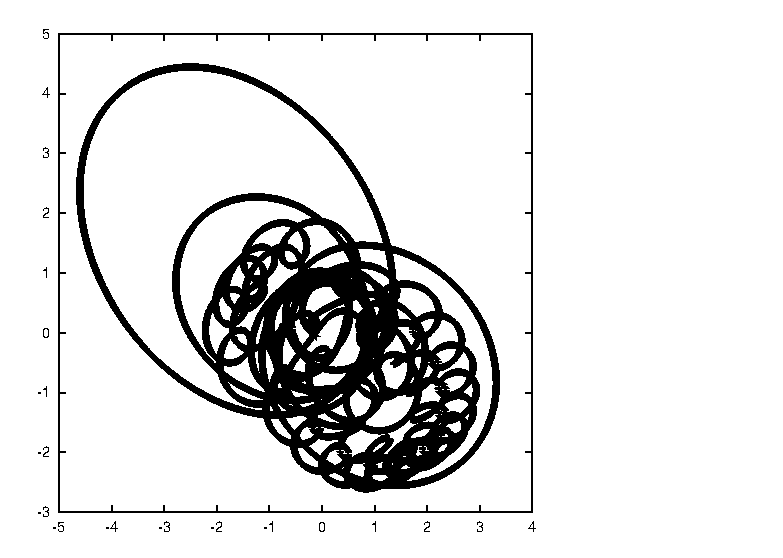
\includegraphics[width=2.5in]{chap5/leapfrog2a_0.00001_100.ps}
\caption[Three stars on a circle, leapfrog, $dv_{init}=0.0001$, $dt = 0.00001$,
$t_{end} = 100$]
{The fifth attempt to integrate the orbits of three stars
starting off on a circle with an initial velocity perturbation of 
$dv_{init}=0.0001$, time step $dt = 0.00001$ and a total duration of
$t_{end} = 100$}
\label{fig:leap2a-0.00001-100}
\end{figure}

\abc

\bob
Surprise!  Virtually the same picture, all of a sudden!  So now I
agree that Alice was really right on both counts.  But I have one last
worry.  Why has the energy error suddenly shrunk so much, by a factor
of more than a thousand, where I would have expected only a hundred?

\alice
Hard to say.  In the two-body case it was not so hard to track down
all aspects of the integration errors, since the underlying orbits
were so simple.  But look here, what a mess!  In order to answer
your last worry, we need to build a lot more tools.  Besides a switch
to variable time steps in the integrator, which we'll get around to at
some point, we need much better ways to dissect orbit segments, in
order to focus on particularly interesting interactions.  Ideally, we
would like to build in some form of artificial intelligence, so that
the particles themselves will know how to take notes while they are
flying around and being flung around.  When we can harvest their
stories at the end of an integration, we will have a head start in
answering questions of the type you asked.  You'll have to be a bit
patient though, since it will require quite a number of sessions to
get to that point.

\carol
Well, I'm game.  It's a lot of fun already, to see how much progress
we have made.  The fact that we have now reached a point where we can
ask questions that call for some form of artificial intelligence to
answer them is impressive enough.  Besides, it means that I, too,
might start to write a working paper about part of what we are doing
now.  One footnote, though: I wouldn't call these orbits a mess; on
the contrary, I find all this wheeling around quite elegant.

\bob
Elegance is in the eye of the beholder, I guess, but I must admit that
I, too, find this figure skating quite pretty.  And I am desperately
thinking how I could make a working paper out of all this --- perhaps
for an art class?

\alice
When I called the orbits a mess, I meant it in an affectionate way.
It reminded me of my room, which I haven't cleaned up for a while, but
that's another story.  How about inviting more art, and running this
thing for a hundred million time steps, by going to {\st t\_end = 1000}?

\bob
You have my blessing.

\cba

\begin{small}
\begin{verbatim}
|gravity> leapfrog2a > leapfrog2a_0.00001_1000.out
Please provide a value for the time step
0.00001
and for the duration of the run
1000
Initial total energy E_in = -0.866025
Final total energy E_out = -0.866025
absolute energy error: E_out - E_in = -5.78748e-10
relative energy error: (E_out - E_in) / E_in = 6.6828e-10
|gravity>
\end{verbatim}
\end{small}

\section{The End of the Story}

When Alice plotted the resulting picture, they were all surprised to
see an almost one-dimensional plot, barely visible on the screen.
There seemed to be two particles moving away from the center, one
reaching $y=160$ on top, and one reaching $y=-320$ below.  The
tick marks and labels on the $x$ axis were so compressed, they were not
even readable.

Alice then pointed out that it was likely that there had been a close
near-simultaneous three-body encounter, from which two stars emerged
as a tight double star, a binary in astrophysical terms.  Since a
tight binary has a large negative binding energy, the remaining
positive energy has to be carried away by the third star.  Since we
are plotting orbits in the c.o.m. frame, the direction of the single
star's escape orbit must be exactly opposite from the direction of the
escape orbit of the double star.  And since the latter carries twice
as much mass as the single star, its speed in the c.o.m. frame has to
be half as large as that of the star escaping by itself.  This explains
why the track moving downwards has reached twice as large a distance
from the origin as the track moving upwards.  Although not visible in
the terribly skinny figure, the upwards track must be that of the
binary, and the downwards track that of the single star.

Given the large distance that the stars had traveled, Alice decided to
be more conservative, and try to run the simulation for only 200 time
units, rather than 1,000.  Here is her result:

\begin{small}
\begin{verbatim}
|gravity> leapfrog2a > leapfrog2a_0.00001_200.out
Please provide a value for the time step
0.00001
and for the duration of the run
200
Initial total energy E_in = -0.866025
Final total energy E_out = -0.866025
absolute energy error: E_out - E_in = 9.36223e-11
relative energy error: (E_out - E_in) / E_in = -1.08106e-10
|gravity>
\end{verbatim}
\end{small}

The accompanying plot she made was still very skinny.  They at least
could see a few tick marks below along the $x$ axis, though all the
numbers there were still printed on top of each other.  The upwards
track reached $y=23$, while the downwards track extended to $y=-46$.
And indeed, the upwards track could now be seen to be slightly thicker
than the downwards track, in agreement with Alice's prediction that
that one was formed by the two stars in a tight binary.

Again shortening the duration of the run, Alice let the stars run to
{\st t\_end = 150}:

\begin{small}
\begin{verbatim}
|gravity> leapfrog2a > leapfrog2a_0.00001_150.out
Please provide a value for the time step
0.00001
and for the duration of the run
150
Initial total energy E_in = -0.866025
Final total energy E_out = -0.866025
absolute energy error: E_out - E_in = 1.02107e-09
relative energy error: (E_out - E_in) / E_in = -1.17903e-09
|gravity>
\end{verbatim}
\end{small}

And still the plot looked skinny!  Most of the interaction region in
the center resembled a single ink blob, and the two tracks now reached
to $y=13$ and $y=-26$, respectively.  They concluded that the close
encounter leading to the double escape must have taken place soon
after {\st t = 100}.  The reasoning was as follows: if the stars would
move in straight line in uniform motion, an extrapolation of the last
two results would lead to two short tracks already having started at 
{\st t = 100}, reaching $y=3$ and $y=-6$, respectively.  However, the
particles are decelerating, due to the gravitational interaction
between the single star and the double star.  Therefore, the initial
separation must have happened at a higher speed, moving the time of
the close three-body encounter further toward the future, most likely
around or slightly after {\st t = 100}.

To check this reasoning, Alice produced an even shorter run, this time
only to {\st t = 120}:

\begin{small}
\begin{verbatim}
|gravity> leapfrog2a > leapfrog2a_0.00001_120.out
Please provide a value for the time step
0.00001
and for the duration of the run
120
Initial total energy E_in = -0.866025
Final total energy E_out = -0.866025
absolute energy error: E_out - E_in = 1.48818e-11
relative energy error: (E_out - E_in) / E_in = -1.7184e-11
|gravity>
\end{verbatim}
\end{small}

This finally produced a reasonable plot, with readable numbers along
the $x$ axis:

\begin{figure}[htb]
\centering
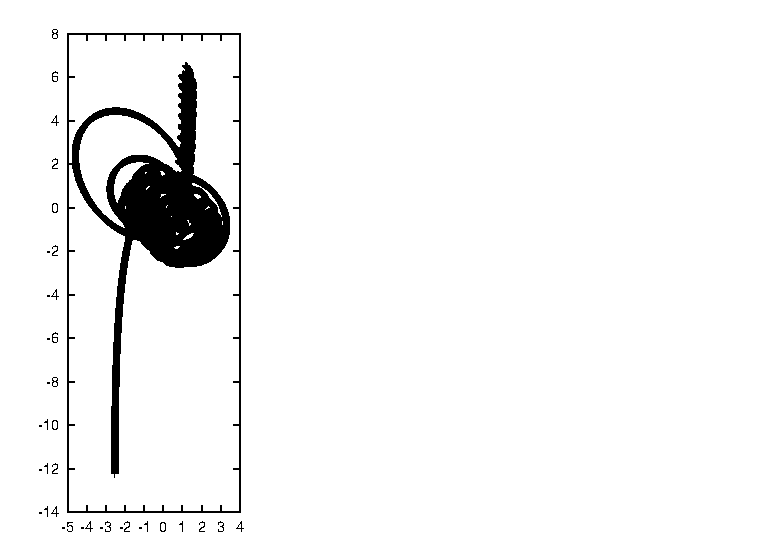
\includegraphics[width=2.5in]{chap5/leapfrog2a_0.00001_120.ps}
\caption[Three stars on a circle, leapfrog, $dv_{init}=0.0001$, $dt = 0.00001$,
$t_{end} = 120$]
{The ninth attempt to integrate the orbits of three stars
starting off on a circle with an initial velocity perturbation of 
$dv_{init}=0.0001$, time step $dt = 0.00001$ and a total duration of
$t_{end} = 120$}
\label{fig:leap2a-0.00001-120}
\end{figure}

Looking back at the three overly skinny plots, not shown here, and
using the numbers they read off as reported above, our friends noticed
that the separation between binary and single star at time {\st t = 1000}
was about seven times larger than at time {\st t = 200}.  Uniform motion
would have predicted an increase of separations by a factor nine.  The
actual factor seven was recognized as evidence that the relative
motion between single star and binary was still slowing down.  The
question was raised whether the stars would fall back again eventually,
or whether they would really escape in opposite directions.  To answer
this question, their was no need for an extra plot.  They just ran a
run of a billion time steps (which took a while) and tossed out all but
the last few lines of the output:

\begin{small}
\begin{verbatim}
|gravity> leapfrog2a | tail
Please provide a value for the time step
0.00001
and for the duration of the run
10000
Initial total energy E_in = -0.866025
Final total energy E_out = -0.866025
absolute energy error: E_out - E_in = 6.29064e-09
relative energy error: (E_out - E_in) / E_in = -7.26381e-09
-68.4785 1632.06 0 -0.137523 -0.382285 0 
137.396 -3263.57 0 0.0141025 -0.325753 0 
-67.9165 1631.51 0 0.112159 0.719282 0 
-68.4798 1632.06 0 -0.126162 -0.39353 0 
137.396 -3263.57 0 0.0141025 -0.325753 0 
-67.9154 1631.51 0 0.100483 0.73056 0 
-68.481 1632.05 0 -0.114485 -0.404807 0 
137.397 -3263.57 0 0.0141025 -0.325753 0 
-67.9145 1631.52 0 0.0884761 0.741873 0 
-68.4821 1632.05 0 -0.102479 -0.41612 0 
|gravity>
\end{verbatim}
\end{small}

This proved clear evidence for final escape of both binary and single
star.  Whereas the single star had separated from the binary by a
distance of 320+160=480 units along the $y$ axis at {\st t = 1000},
the separation had now increased to about 4900 units, in a roughly
eleven times longer interval, counted from the slingshot event around
{\st t = 100}.  The conclusion was that there had been some residual
slowing down, given that the separation had increased by a factor ten
rather than eleven, but that escape had been established, since there
was no indication that the slow-down would be enough to lead to a fall
back.

After concluding once that it was high time to write better analysis
tools, which would allow a more direct investigation of the questions
they had now answered in a somewhat haphazard way, our friends called
it quits for that night.

\section{Three Bodies on a Figure Eight}

The next time Alice, Bob, and Carol met, they decided to make one more
modification to their 3-body version of the leapfrog code, before
going to a more modular and flexible $N$-body version.  Alice had
mentioned a relatively recent discovery of a new solution to the
centuries old three-body problem, in the form of three stars of equal
mass following each other along a single orbit resembling a figure eight.
Here is the first half of the code, which lists the initial conditions,
followed by the computation of the initial accelerations as well as
kinetic and potential energy.  The second half of the code is
identical to the second half of {\st leapfrog2.C}.

\code{leapfrog3.C: first half}{chap5/leapfrog3.C.first_half}

They first tried their standard time step choice {\st dt = 0.01} for a
integration until {\st t\_end = 100}:

\begin{small}
\begin{verbatim}
|gravity> g++ -o leapfrog3 leapfrog3.C
|gravity> leapfrog3 > leapfrog3_0.01_100.out
Please provide a value for the time step
0.01
and for the duration of the run
100
Initial total energy E_in = -1.28705
Final total energy E_out = -1.28706
absolute energy error: E_out - E_in = -1.25936e-05
relative energy error: (E_out - E_in) / E_in = 9.78486e-06
|gravity>
\end{verbatim}
\end{small}

\begin{figure}[htb]
\centering
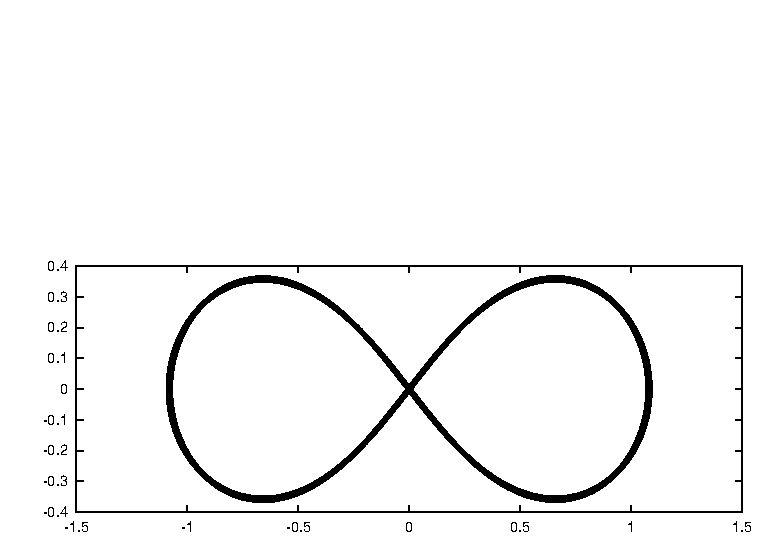
\includegraphics[width=4.5in]{chap5/leapfrog3_0.01_100.ps}
\caption[Three stars on a figure-8 orbit, $dt = 0.01$,
$t_{end} = 100$]
{The first attempt to integrate the orbits of three stars
starting off on a figure-8 orbit with time step $dt = 0.01$ and a
total duration of $t_{end} = 100$}
\label{fig:leap3-0.01-100}
\end{figure}

Even though the energy error was not that small, no deviation in the
orbit was visible.  Clearly, the three-body figure-8 orbit is far more
stable than the three-body circular orbit, which fell apart well
before reaching 100 time units, as we saw before.  Taking a ten times
smaller time step neatly decreased the errors by a factor of one hundred,
also a good sign of reaching convergence in the orbits:

\begin{small}
\begin{verbatim}
|gravity> leapfrog3 > leapfrog3_0.001_100.out
Please provide a value for the time step
0.001
and for the duration of the run
100
Initial total energy E_in = -1.28705
Final total energy E_out = -1.28705
absolute energy error: E_out - E_in = -1.19725e-07
relative energy error: (E_out - E_in) / E_in = 9.30233e-08
|gravity>
\end{verbatim}
\end{small}

When plotting this last result, it looks exactly like
Fig. \ref{fig:leap3-0.01-100}, so we will omit it here.

Our friends then repeated the second test for instability, by `priming
the pump' again, with an offset of $10^{-4}$ in the $x$ component of
the first particle.  As before, they added the one line

\begin{small}
\begin{verbatim}
    v[0][0] += 0.0001;
\end{verbatim}
\end{small}

\noindent
immediately following the assignment of velocities at the beginning of
the program.  They renamed this modified code {\st leapfrog3a.C}.
Here is what happened by {\st t\_end = 100}:

\begin{small}
\begin{verbatim}
|gravity> g++ -o leapfrog3a leapfrog3a.C
|gravity> leapfrog3a > leapfrog3a_0.001_100.out
Please provide a value for the time step
0.001
and for the duration of the run
100
Initial total energy E_in = -1.287
Final total energy E_out = -1.287
absolute energy error: E_out - E_in = -1.27819e-07
relative energy error: (E_out - E_in) / E_in = 9.93155e-08
|gravity>
\end{verbatim}
\end{small}

\begin{figure}[htb]
\centering
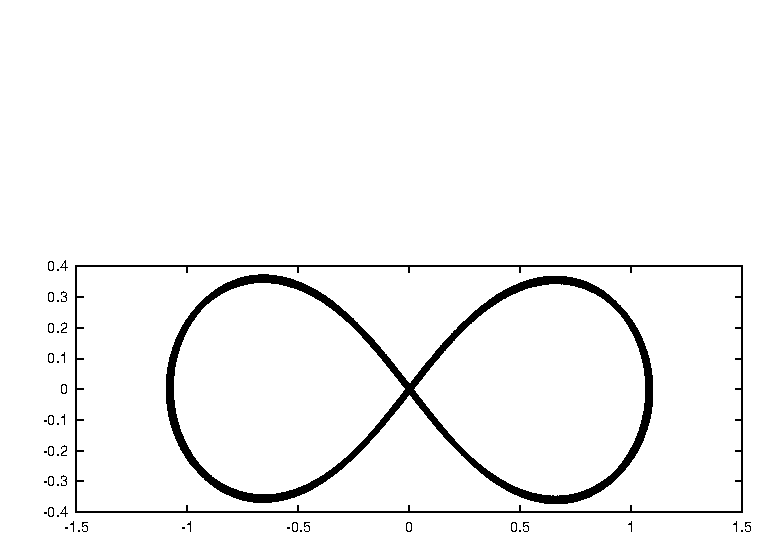
\includegraphics[width=4.5in]{chap5/leapfrog3a_0.001_100.ps}
\caption[Three stars on a figure-8 orbit, $dv_{init}=0.0001$, $dt = 0.001$,
$t_{end} = 100$]
{The first attempt to integrate the orbits of three stars starting off
on a figure-8 orbit with an initial velocity perturbation of
$dv_{init}=0.0001$, time step $dt = 0.001$ and a total duration of
$t_{end} = 100$}
\label{fig:leap3a-0.001-100}
\end{figure}

Again, no visible deviations, very similar small energy errors, and no
sign of any instability.  This confirms what has been described in the
literature, that the figure-8 orbit for three bodies is stable.

We leave it as an exercise for the reader to explore when and how the
figure-8 configuration falls apart (or perhaps winds up in a higher
order version of a stable orbit, with more loops and turns) upon an
increase of the magnitude of the perturbation, either in one of the
velocity components or in one of the position components, or in a mix
of perturbations of various position and velocity components.
